\graphicspath{{Chapter4/Chapter4Figs/}}

\chapter{Systems biology for investigating mTOR network in ageing}
\label{chap:Systems biology for investigating mTOR network in ageing}
This chapter begins by presenting the main concepts of systems biology, from parameter estimation to advanced techniques of dynamical system theory. Finally, published work on systems modelling of the mammalian TOR network are described.

\section{Introduction to systems biology}
\label{sec:Introduction to systems biology}
Understanding the connections between proteins to form networks and determining the emergent properties of dynamical interactions has been a major focus of research in recent years. Due to the complexity of biological systems, the need for an appropriate level of abstraction in order to characterise the key signalling network governing cell behaviour is essential. An approach to address the problem is provided in the mathematical modelling of signalling pathways \citep{Kolch2005, Hughey2009}. So far, several key pathways have been modelled and simulated such as the epidermal growth factor (EGF) pathway \citep{Borisov2009, Schilling2009, Wang2009}, the insulin insulin-like pathway \citep{smith2010foxo_modelling, Brannmark2010, Nyman2012} or p53/MDM2 oscillation signalling \citep{GevaZatorsky2006, Proctor2008}. This chapter presents a concise introduction to systems biology and other more advanced techniques imported from dynamical systems theory with the aim of introducing the current mathematical models of 
the TOR network.\\

\subsection{Why systems biology?}
\label{subsec:Why systems biology?}
Before introducing the main concepts important for dynamic modelling in systems biology, I think it is reasonable to discuss what systems biology is and how it can improve our understanding in biological studies. Systems biology is not simply a means to replace expensive wet-experiments with dry alternatives. It would not be very useful to consider systems biology just as an additional tool to provide more evidence to support scientific findings. From this point of view, a systems biology approach does not reveal much more than using wet-experimental techniques.\\ 
The advantages of systems biology are multiple. Firstly, the system representation is an abstraction of the biological context, and therefore it is simpler to investigate. Systems biology offers an extraordinary possibility to represent our biological knowledge as an interconnected system using an appropriate formalism. Secondly, this system can be formally analysed from multiple perspectives using theories coming from other sciences such as mathematics and computer science (e.g. dynamical systems, optimisation, formal methods), and statistics (e.g. stochastic simulation of models). Thirdly, from these analyses, specific properties of the system can be extracted and formulated as modelling predictions which can be tested in the laboratory. Systems biology permits the biologist to selectively search those predictions (e.g. systematic sensitivity analysis of system components) as well as provides the user with new non-trivial results (e.g. system bifurcations at specific protein amounts). Moreover, the 
feasibility of obtaining these predictions is mainly due to fast numerical computing tools, which allows the user to perform high-throughput tasks which would be impossible for wet-experimentalists. 

\subsection{Model definition}
\label{subsec:Model definition}
Over the last 20 years, the necessity of creating a standard language for systems biology models has emerged. Systems Biology Markup Language (SBML) \citep{hucka2003systems} was developed as an XML standard aimed at porting systems biology models amongst different platforms and therefore increasing systems biology interoperability. In the field of molecular systems biology, a model is described as: (1) a set $S$ of species (e.g. unphosphorylated or phosphorylated proteins, complexes), (2) a set $R$ of reactions between species (e.g. phosphorylation, binding), (3) a set $I$ of inputs (e.g. insulin stimuli), and (4) a set $C$ of compartments (e.g. cytoplasm, nucleus). These biological models can be graphically represented using CellDesigner\footnote{\href{http://www.celldesigner.org/}{http://www.celldesigner.org/}} \citep{Funahashi2003, Funahashi2008}. Although this representation can be user-friendly, it hides the real representation of a model from a mathematical point of view. Instead, a mathematical 
representation explicitly offers the details for dealing with tasks such as parameter estimation and model quality analysis. A biological model can be described as follows:
\begin{align}
  \dot{\vec{x}}_{t,\theta} &= \vec{f}(\vec{x}_{t,\theta},\vec{u}_{t,\theta},\theta),\;\;\; \vec{x}_{t_{0},\theta} = \vec{x}_{0,\theta} \label{eq:ode_system} \\
  \vec{y}_{t,\theta} &= \vec{g}(\vec{x}_{t,\theta},\theta) + \vec{\epsilon} \label{eq:observable_function}
\end{align}
where \ref{eq:ode_system} is a system of Ordinary Differential Equations (ODEs) and \ref{eq:observable_function} describes the model observable variables. The ODE-based model is characterised by $n$ species $\vec{x}$ (e.g. protein concentrations), whose dynamics are dependent on $l$ input functions $\vec{u}$ (e.g. constant or impulse stimulation) and $j$ model parameters $\theta = \{\theta_1,\dots,\theta_j\}$ (e.g. protein initial concentrations, kinetic rates constants, scaling factors) over time $t = \{0,\dots,T\}$. The species in $\vec{x}$ which can be experimentally measured (e.g. by immunoblotting, mass spectrometry), are mapped into $m$ observable variables $\vec{y}$ by an observable function $\vec{g}$ and a measurement error $\epsilon \approx N(0,\sigma^{2}(d_{i,k}))$, where $\sigma^{2}(d_{i,k})$ is the variance of the $i$-th measurement at the time point $k$.

\subsection{Parameter estimation}
\label{subsec:Parameter estimation}
The choice of the observable variables depends on the measurements that can be feasibly measured in the laboratory. Once these  are collected, the model can be optimised in order to represent the experimental data within a certain error. Parameter estimation is the task in which the model parameters are established in order to reduce this error. Let ${d}_{i,k}$ and 
$y_{i,k,\theta}$ be the $i$-th data measurement and observable at the time point $k$ respectively, and $\sigma(d_{i,k})$ be the standard deviation for $d_{i,k}$, parameter estimation aims at measuring the distance between the model observables and the experimental data:
\begin{equation}
  \label{eq:chi_square}
  \chi^{2}(\theta) = \sum_{i=1}^{m} \sum_{k=0}^{T} \left(\frac{d_{i,k} - y_{i,k,\theta}}{\sigma(d_{i,k})}\right)^{2}
\end{equation}
and computing a solution, or assignment of values to the parameters $\theta$, which minimises such a distance:
\begin{equation}
  \label{eq:hat_theta}
  \hat{\theta} = \argmin_\theta {(\chi^{2}(\theta))} 
\end{equation}
Parameter estimation is therefore a problem of minimum optimisation. Optimisation algorithms can be classified into two classes: global and local algorithms. Global optimisation algorithms aim at finding the solution of minimum cost\footnote{Maximum cost in the case of maximum optimisation.} in the differential $\chi^2$ manifold\footnote{An $n$-dimensional manifold is a topological space having the property that the neighbourhood of each point approximates (formally, it is \emph{homeomorphic} to), the Euclidean space of dimension $n$, whereas this may not hold true globally.} $\mathcal{M}$ of the search space. Although these algorithms can be very accurate since the performed research is more extended, they usually have exponential time complexity. An additional problem is that they can stall on local minima, which may not be suitable as solutions. Examples of these algorithms are simulating annealing (SA) \citep{Kirkpatrick83, Corana1987}, genetic algorithms (GA) \citep{Baeck1993, Michalewicz1994, 
Mitchell1998, Baeck1997} and evolutionary programming (EP) \citep{Fogel1992, Baeck1993, Baeck1997}. Local optimisation algorithms focus on retrieving the minimum solution closest to the current assignation of parameter values. These algorithms usually permit to calculate a solution quickly, although this may not be optimal. Instances of this class are Trust Region (TR) \citep{Celis1984, Byrd1987, Yuan2000}, Levenberg-Marquardt (LM) \citep{Levenberg1944, Marquardt1963}, Steepest Descent (SD) \citep{Fogel1992} and Truncated-Newton (TN) \citep{Gill1981, Nash1984}. A common approach is to perform a global optimisation and then improve the solution quality by a local optimisation. These methods are implemented in several software tools for calibrating and analysing systems biology models. The models presented in this thesis were developed using Copasi\footnote{\href{http://www.copasi.org/}{http://www.copasi.org/}} \citep{Hoops2006} and the Matlab toolboxes Potterswheel\footnote{\href{http://www.potterswheel.de/}{
http://www.potterswheel.de/}} \citep{Maiwald2008, Hengl2007, Raue2009} and SBToolbox2\footnote{\href{http://www.sbtoolbox2.org/}{http://www.sbtoolbox2.org/}} \citep{Schmidt2006}. 
In the case of testing different biological hypotheses, each corresponding to a specific network structure, parameter estimation can be used for establishing a rank within these different networks, based on fitting quality. The $\chi^2$ measure is sufficient to define this hypothesis rank if the number of parameters is the same for each model, otherwise other measures taking into account the number of parameters, such as Akaike information criterion (AIC) \citep{Akaike1973} or Bayesian information criterion (BIC) \citep{Schwarz1978}, should be adopted. This hypothesis ranking can be useful as a means to predict likely network structure and to guide further experimental test that could discriminate between alternatives. An example of this approach can be found in \citep{Sonntag2012}.

\subsection{Identifiability analysis}
\label{subsec:Identifiability analysis}
In parameter estimation, two problems arise depending on model structure and data availability. The former concerns model structural non-identifiability \citep{Bellu2007, Raue2009, Raue2010, Balsa-Canto2010, Chis2011}. This type of non-identifiability happens when the model structure is not sufficiently mapped by the available data. For instance, if a sub-graph of the network is over-parameterised or there are not sufficient observables characterising those dynamics, that sub-component may result structurally non-identifiable. From a graphical point of view, structural non-identifiability is represented in the $|\theta|$-dimensional $\chi^2$ space as an unlimited plateau along the dimensions of the structurally non-identifiable parameters. Formally, assuming absence of measurement noise $\vec{\epsilon} = 0$, a subset of parameters $\eta \subset \theta$ is structurally non-identifiable if the overall $\chi^2$ remains constant for each assignment $a \in A$ to the parameters in $\eta$:
\begin{equation}
  \label{eq:structural_nonidentifiability_1}
  \{\forall \; \eta := a \; | \; \eta \subset \theta, a \in A\} \Rightarrow \chi^2(\theta) = const
\end{equation}
In other words, the parameters in $\theta$ cannot be uniquely determined due to a lack of observable information:
\begin{equation}
  \label{eq:structural_nonidentifiability_2}
  \vec{y}_{t,\eta} = \vec{g}(\vec{x}_{t,\eta},\eta) = \vec{0} \Rightarrow \chi^2(\theta) = const
\end{equation}
In practical terms, if a model is structurally non-identifiable, parameter estimation results are inconclusive, as infinite different solutions report the same $\chi^2$. Structural identifiability can be solved by altering the model structure or increasing the numbers of observable variables for the structurally non-identifiable sub-graph. Among the software for testing structural identifiability, the software GenSSI\footnote{\href{http://www.iim.csic.es/~genssi/}{http://www.iim.csic.es/$\sim$genssi/}} \citep{Balsa-Canto2010, Chis2011} was used in this thesis. GenSSI computes the successive $k$ orders of Lie derivatives of $\vec{g}$ with respect to the vector field $\vec{f}$, evaluated at the initial time $t=t_0$. In this generating series approach, GenSSI searches for a \emph{exhaustive summary}, which is a vector of the series coefficients, evaluated at the initial conditions, that only depends on the model parameters to estimate and identify. Then, GenSSI uses the exhaustive summary for computing 
solutions for the parameters $\theta$. If a unique solution is found, then the parameters are structurally globally identifiable; in the case of multiple solutions, the parameters are structurally locally identifiable. Finally, in the case of no solution, the parameters are structurally non-identifiable. \\
% GenSSI computes the successive $k$ orders of Lie derivatives of $\vec{g}$ 
%with respect to the vector field $\vec{f}$, evaluated at the initial time $t=t_0$:
% \begin{equation}
%   \label{eq:structural_nonidentifiability_3}
%   L_{\vec{f}_0} \dots L_{\vec{f}_k} \; \vec{g}(\vec{x}_{t, \theta},\theta, t)
% \end{equation}
% where such a Lie derivative is defined as:
% \begin{equation}
%   \label{eq:structural_nonidentifiability_4}
%   L_{\vec{f}} \; \vec{g}(\vec{x}_{t, \theta},\theta, t) = \sum_{j=1}^{n_x} 
%f_j(\vec{x}_{t, \theta}, \theta, t) \frac{\partial \vec{g}(\vec{x}_{t, \theta}, \theta, t)}{\partial x_{t, \theta, j}}
% \end{equation}
% Therefore, a model is structurally identifiable at Lie derivative of order $i$ if 
%a unique solution for $\theta$ can be obtained from the algebraic equation for $L_{\vec{f}_i}$. \\
Although a parameter is structural identifiable, it may still be practically non-identifiable \citep{Raue2009, Raue2010}. Practical non-identifiability depends on the amount or quality of data sets used to estimate model parameters and can therefore be solved by increasing or improving the measured data. In case of time-course-based experiments, this means that the collected time points are not enough in number or that their standard deviations are too big to allow the optimisation algorithm to infer clear time-dependent signalling trajectories. Therefore, practical identifiability concerns the problem of assessing finite confidence intervals for each parameter. A parameter $p$ is practically non-identifiable when its confidence interval is infinite, although there may exist a unique minimum for it. Graphically, the $\chi^2$ measured as a function of $p$, $\chi^2(p)$, is always lower than a desired confidence threshold $\Delta_\alpha$, in the neighbourhood of the parameter minimum $p_m$:
\begin{align}
  \label{eq:practical_nonidentifiability}
  \forall \; \delta \in \mathbb{R}^{+}: \; &\{\chi^2(p:=p_m) \le \chi^2(p:=p_m \pm \delta)\}, \\
  &\{\chi^2(p:=p_m - \delta) < \Delta_\alpha \vee \chi^2(p:=p_m + \delta) < \Delta_\alpha \} \notag 
\end{align}
This results in a deficiency in estimating a valid confidence interval for $p$ \citep{Raue2009, Raue2010, Raue2011, Kreutz2012}. A problem with this approach regards the choice of $\Delta_\alpha$. This threshold is defined as $\Delta_\alpha = \chi^2(\alpha, df)$, where $\chi^2(\alpha, df)$ is the $\chi^2$-distribution with confidence level $\alpha$ and degrees of freedom $df$ which corresponds to the number of parameter estimations. Therefore, an accurate $\Delta_\alpha$ depends on a sufficiently large number of precise parameter estimations which requires a considerable time to compute.\\ 
% Unfortunately, (1) the search space can contain several local minima and 
%(2) an optimisation algorithm can fail the convergence especially in the case of local optimisation algorithms. Whereas the second issue can be partially solved using global 
%optimisation algorithms, the first issue cannot be easily solved except by increasing 
%the amount of data, which augments the constraints in the parameter search space. 
%All these parameter estimations are included in the computation of $\Delta_\alpha$, 
%although several of them may not be reasonably accepted. This counting increases 
%the number of degrees of freedom for the $\chi^2$-distribution, leading to a reduction 
%of its variance, an increment of its the mean and a better approximation to a normal 
%distribution. As consequence, the threshold $\Delta_\alpha$ may result higher than 
%what is already sufficient for defining a confidence interval and therefore showing 
%the parameter as practically non-identifiable whereas it may be instead. 
%This situation is particularly likely in models with high number of parameters 
%because the parameter search space may dramatically increase its non-linearity 
%and therefore the number of local minima. For this reason, practical non-identifiability 
%was not investigated in the studies presented in this work. \\
In this thesis, the Potterswheel plugin Mean Optimal Transformations Analysis (MOTA) \citep{Hengl2007} was employed for detecting functionally related parameters and therefore solving structural non-identifiability issues in relation with data sets adopted for parameter estimation, in conjunction with a structural identifiability analysis theoretically performed using GenSSI. From a fit sequence of parameters, the MOTA algorithm returns the tuples of highly related parameters, permitting the user to fix independent parameters and estimate the remaining related parameters in the \emph{reduced} parameter space. These iterations of parameter estimation and fixing may eventually terminate leading to model identifiability, decreasing the variability of estimated parameters. In order to provide the user a graphical intuition of identifiability issue, Figure \ref{fig:landscape_identifiability} illustrates parameter non-identifiability through graphical $\chi^2$ landscape surface.

\subsection{Model simulation}
\label{subsec:Model simulations}
Before introducing a definition for simulation and describing the operations which can be done over a simulation, it is worth formalising the concept of algorithm. An algorithm $\mathcal{A}$ is a step-by-step procedure with an internal state $\mathcal{S}$ which receives an input $\mathcal{I}$, performs a list of instructions evolving $\mathcal{S}$ and returns an output $\mathcal{O}$ \citep{Cormen2009}:
\begin{equation}
  \label{eq:algorithm_definition}
  \mathcal{A}: (\mathcal{I},\mathcal{S}) \longrightarrow \mathcal{O}
\end{equation}
Therefore, a simulation can be defined as the task of reproducing a real problem, using an algorithm \citep{Malesani2004}. In this context, the interest is in simulating aspects of cellular behaviour, formally represented by mathematical models, and collecting information related to their temporal evolution. A mathematical model can be simulated deterministically or stochastically, depending on the type of algorithm used for reproducing its dynamical behaviour. 
For a certain input, a deterministic algorithm always returns the same output, reproducing the same internal state sequence. In other words, a deterministic algorithm does not contain any form of randomisation. An example of these algorithm is LSODA \citep{Hindmarsh1983, Petzold1983}. Stochastic algorithms differ as they include some form of randomisation, defined by a specific probability distribution, in their procedure \citep{Wilkinson2006}. This randomisation can be limited to the internal state sequence only or be propagated to the output. In the former case, a stochastic algorithm is called \emph{Las Vegas}\footnote{An instance of this class of algorithm is Randomised-Quicksort.} (LV), whereas in the latter case the algorithm is named \emph{Monte Carlo} (MC) \citep{Motwani1995, Cormen2009}. In the context of systems biology, the stochasticity of a biological context can be reproduced by MC stochastic algorithms, such as Gillespie \citep{Gillespie1976}, Gibson-Bruck \citep{Gibson2000}, Tau-Leap \citep{
Rathinam2003} or Runge-Kutta \citep{Kloeden1999}. This is of particular importance in the case of modelling gene transcription or low levels of protein amounts, since these systems are highly stochastic. The major drawback of stochastic simulations is their long computation-time as compared to deterministic simulations. For this reason, if the system stochasticity is low, a deterministic simulation may be more convenient for representing the dynamical behaviour of the model.

\subsection{Sensitivity analysis}
\label{subsec:Sensitivity analysis}
In mathematical modelling, establishing the influence of the parameters on overall behaviour is of fundamental importance to understand which of them play a more significant role then others \citep{Aldridge2006}. The analysis addressing this question is called sensitivity analysis. Sensitivity analysis is particularly useful in several areas. For instance, the detection of irrelevant parameters on the global dynamics may suggest model reduction \citep{Jia2008}, whereas assessing important ones may lead to new experimental design \citep{Cho2003}. Sensitivity analysis offers a means to explore the robustness of a system, as it shows how the dynamics change depending on parameter perturbation. There exist two types of sensitivity analysis: global and local. Global sensitivity analysis aims at retrieving multidimensional sensitivity operating multiple parameter changes. Local sensitivity analysis aims at exploring the domain of one parameter only and analysing the effect on the others \citep{Marino2008}.\\
The main concepts of sensitivity analysis are presented limiting the objective to linear models \citep{Saltelli2005}. A linear model can be represented as 
\begin{equation}
   \label{eq:linear_model}
   Y = \sum_{i=1}^{n} \Omega_i Z_i
\end{equation}
where $Y$ is the model output, $Z_i$ are uncertain input factors chosen from a normal distribution $Z_i \approx N(0,\sigma_{Z_i})$ and $\Omega_i$ are the coefficients for $Z_i$. $Y$ is also normally distributed $Y \approx N(0,\sigma_{Y})$, where $\sigma_Y = \sqrt{\sum_{i=1}^{n} \Omega_i^2 \sigma_{Z_i}^2 }$. Therefore, measuring a normalised sensitivity of $Z_i$ over $Y$ can be defined as:
\begin{equation}
  \label{eq:sensitivity_analysis}
  S_{Z_i}^{\sigma} = \frac{\sigma_{Z_i}}{\sigma_{Y}}\frac{\partial Y}{\partial Z_i}
\end{equation}
In case of a non-linear model, an extension of the previous calculation of sensitivity analysis based on MC methods can be found in \citep{Cho2003, Saltelli2005, Saltelli2008}.\\
Sensitivity analysis can be used in combination with model simulation. In fact, model simulations become particularly interesting when the initial conditions, such as the initial protein amounts or input stimuli, are changed. This type of simulation can reveal specific predictions, which can then be tested experimentally. For instance, reducing the amount of a protein species corresponds to a simulated knock-down, whereas increasing it represents a simulated over-expression. In the field of systems biology, cases of study involving this type of approach are \citep{Babu2004, Ihekwaba2004, Mahdavi2007, DallePezze2012a}. In this work, the term \emph{model perturbation} will be used to refer to a generic alteration of protein amount. Model perturbations can be interpreted as local sensitivity analyses performed on target species by varying their expression level. Of course, the number of protein species perturbed is not necessarily limited to one at a time. In fact, an advantage of systems modelling is the 
possibility to compute these dry-experiments relatively easily compared to wet-experiments in a laboratory. These predictions may reveal non-trivial dynamical changes at certain time points as well as at specific protein levels. Therefore, a biologist may use this information for reducing the number of experiments, as models can return optimal conditions for detecting differences or similarities, and extending biological knowledge, as models can predict completely new system behaviours. 

\section{Advanced analyses from dynamical systems theory}
\label{sec:Advanced analyses from dynamical systems theory}
Dynamical systems theory constitutes a powerful body of knowledge which can be used to investigate dynamical properties of the model. This section presents some of these analyses and their importance in the study of biological models.
\subsection{Steady-state analysis}
\label{subsec:Steady-state analysis}
After a certain amount of time, a system may reach a state characterised by invariability. This state is called steady state. A definition of steady state based on \citep{Garg2007, Ay2009} can be proposed as follows. Let $S$ be a set of states. $\forall s_i \in S$, $s_i$ is steady if and only if the following two conditions are verified:
\begin{align}
\label{eq:steady_state_analysis}
 1.\;\; & Succ(S) = S \\
 2.\;\; & \forall\; s_i,s_j \in S,\;\; \forall\; t \in T\;|\; t : s_i \rightarrow s_j,  \notag \\
        & \exists\; n \in \mathbb{N^{+}} finite \; | \; Prob(t^{(n)}(s_i)=s_i) = 1 \notag  
\end{align}
which means that (1) the set of the successors of $S$ is equal to $S$, and (2) for each visited $s_i \in S$ the probability of re-visiting $s_i$ is $1$ in a finite number of state transitions.\\
In other words, a steady state corresponds to a point at which the system reaches a condition of equilibrium or a fixed point from a mathematical point of view. This analysis is of particular interest for biological systems in order to elucidate the temporal length of specific dynamics and investigate the conditions leading to these steady states. Steady-state conditions also provide scientists with a starting point for analysing system behaviour at such states as illustrated in the following analyses.

\subsection{Stability analysis}
\label{subsec:Stability analysis}
An interesting question arising from the discovery of steady states in a dynamical model regards the system response upon a small perturbation of a steady state. Does this perturbed state move away from or towards its previous steady state? The analysis pertaining to this question is called stability analysis. These sort of questions are of particular interest in biological systems \citep{Thomson2009} and highly relevant in ageing. For example, a senescent cell can be seen as a cell staying in a specific steady state. As stochasticity increases with ageing \citep{FinchKirkwood_book2000, Bahar2006, Kirkwood2008}, the study of stability of a senescent steady state upon stochastic perturbations may reveal important information about the evolution of senescent cells. To provide an intuition of this analysis in the linear case\footnote{In case of non-linear systems, this linearisation technique can still be used although not generally.}, let us consider an $n$-dimensional linear system of ODEs\footnote{For 
simplicity, the Leibniz 
notation of derivative is used here.} \citep{Hirsch2004, Parks1992}:
\begin{align}
  \label{eq:stability_analysis1}
  \frac{dx_i}{dt} &= f_i(x_1, \dots, x_n), \;\;\; (i = 1,\dots, n)
\end{align}
and assume $\vec{s} = (s_1, \dots, s_n)$ be a steady state. Therefore:
\begin{align}
  \label{eq:stability_analysis2}
  f_i(s_1, \dots, s_n)=\frac{ds_i}{dt}=0, \;\;\; \forall\; i\; \in\; [1, n]
\end{align}
This system is now perturbed by a small perturbation $\vec{\rho}=(\rho_1, \dots, \rho_n)$, such that the new perturbed state is $\vec{s}^*=(s_1^*, \dots, s_n^*)=(s_1+\rho_1, \dots, s_n+\rho_n)$.\\
In order to determine whether the perturbed state $\vec{s}^*$ moves away from or towards $\vec{s}$, it is necessary to derive the System \ref{eq:stability_analysis1} at the perturbed state $\vec{s}^*$.
\begin{align}
  \label{eq:stability_analysis3}
  \frac{d(s_i + \rho_i)}{dt} = \frac{d\rho_i}{dt} &= \frac{ds_i^*}{dt}, \;\;\; (i = 1,\dots, n) \;\;\; \text{(by Formula \ref{eq:stability_analysis2})} \\
  &= f_i(s_1^*, \dots, s_n^*) \;\;\; \text{(by definition)}  \notag \\
  &= f_i(s_1+\rho_1, \dots, s_n+\rho_n) \;\;\; \text{(by substitution)}  \notag \\
  &= f_i(s_1, \dots, s_n) + \frac{\partial f_i}{\partial x_1}(s_1,\dots,s_n)\rho_1 + \dots +  \frac{\partial f_i}{\partial x_n}(s_1,\dots,s_n)\rho_n + \mathcal{T} \;\;\; \notag \\ 
  & \text{(Taylor series expansion)}  \notag \\
  &= \frac{\partial f_i}{\partial x_1}(s_1,\dots,s_n)\rho_1 + \dots +  \frac{\partial f_i}{\partial x_n}(s_1,\dots,s_n)\rho_n \;\;\; \text{(by Formula \ref{eq:stability_analysis2})}  \notag
\end{align}
where $\mathcal{T} = \mathcal{O}(\rho_1^n,\rho_2^n,\dots,\rho_1\dots \rho_n)$ are the Taylor series higher-order terms which can be neglected as $\vec{H}$ is assumed a small perturbation. Therefore, the evolution of the perturbation is determined by the following $n$-dimensional linear system:
\begin{align}
  \label{eq:stability_analysis4}
  \begin{pmatrix}
  \frac{d\rho_i}{dt} 
  \end{pmatrix}
 &=
  \begin{pmatrix}
   \frac{\partial f_i}{\partial x_j}(s_1,\dots,s_n)
  \end{pmatrix}
  \begin{pmatrix}
   \rho_i
  \end{pmatrix}, \;\;\; (i, j = 1,\dots, n)\\
 &= J \vec{\rho} \notag
\end{align}
where $J$ is the Jacobian matrix of the System \ref{eq:stability_analysis1} at the fixed point $\vec{s}$. At this stage, it is necessary to calculate the complex \emph{eigenvalues} $\lambda = (\lambda_1, \dots, \lambda_n)$, such that $J \vec{\rho} = \lambda\vec{\rho}$. Let $T = trace(J)$\footnote{The trace of a square matrix is the sum of the elements located on the main diagonal.} and $D = det(J)$, the classification for the fixed point $\vec{s}$ by linear stability analysis is summarised as follows:
\begin{itemize}
 \item Unstable fixed point (repellers or sources): \\$T > 0$, $D > 0$, $\forall \lambda_i \in \lambda: Re(\lambda_i)>0$
 \item Stable fixed point (attractors or sinks): \\$T < 0$, $D > 0$, $\forall \lambda_i \in \lambda: Re(\lambda_i)<0$
 \item Unstable fixed point (saddle points): \\$D < 0$, $\exists \lambda_i \in \lambda: Re(\lambda) > 0$
\end{itemize}
Additional study is required for the case in which there exist at least one eigenvalue with a null real part \citep{Hirsch2004}.


\subsection{Bifurcation analysis} 
\label{subsec:Bifurcation analysis}
Bifurcation analysis offers a way to detect and characterise qualitative behaviour variations around a selected steady state of a model. This leads to the investigation of signal trajectory changes by systematically exploring the domain of one or more model parameters. In conjunction with stability analysis, bifurcation analysis enables one to map the possible states of a system and how this system can switch between them \citep{Aldridge2006}. 
Biological systems are typically characterised by multiple steady states. Therefore, understanding the conditions by which a system transits from one steady state to another one is important, especially when investigating biological states which are apparently irreversible. Many age-related diseases discussed in Section \ref{sec:TOR in age-related diseases} are defined by a cellular dysregulation which denies the system to restore its normal functionality. More generally, since ageing itself has been considered an irreversible process, it would be interesting to investigate under which conditions, a senescent phenotype may \emph{resume} a pre-ageing phenotype or at least remain locked at the current state. Bifurcation analysis provides an exceptional tool for treating and possibly answering these biological questions. Due to the large body of bifurcation theory, this section only provides an overview of it in order to give a graphical interpretation insight of the analysis without dealing with the 
mathematical details. More formal introductions of this theory can be found in \citep{borisuk1997, Hirsch2004}.\\ 
The study of bifurcations concerns the individualisation of \emph{bifurcation points} which are the points corresponding to specific parameter values at which a system undergoes a qualitative state change. A bifurcation is said to be \emph{local} if the bifurcation point is located in the neighbourhood of a fixed point, also called steady-state, or periodic solution, otherwise it is called \emph{global}. The number of parameters which must be specified in order to detect a bifurcation is called \emph{co-dimension}. To clarify these concepts, two instances of bifurcation are graphically represented in Figure \ref{fig:tyson2003_fig1_adapted}. \\
A system containing a bifurcation $b$ can always be reduced to its \emph{normal form}, which is the simplest system preserving $b$. Local bifurcations requires that the perturbation of a parameter alters the stability of a fixed point, that is that the real part of an eigenvalue in $J$ passes through 0\footnote{This typology of fixed points are called non-hyperbolic.}. Because of this, a common approach when working on higher dimensional models consists of calculating the normal form of such a model and then focusing on the \emph{eigenvectors} in the \emph{centre} subspace\footnote{\emph{Centres} are fixed points for which the eigenvalue of $J$ are purely imaginary. For these fixed points, the solution within their subspace do not converge to nor diverge from them.}, ignoring the \emph{stable} and \emph{unstable} subspaces \citep{borisuk1997, borisuk1998}. Conversely, a pragmatic way of mapping the states of a system is by systematically sampling the parameter space and then looking for 
qualitative differences in the phase space \citep{Araujo2007, Wang2010bifurcation}. Of course this approach is only suitable for lower-dimensional models. 

\subsection{Lyapunov exponents} 
\label{subsection:Lyapunov exponents}
When studying a dynamical system, it may be of interest to investigate qualitative behaviour changes over time \citep{Aldridge2006}. A  measure used for characterising this quantity is the vector of \emph{Lyapunov exponents}. This type of analysis allows one to determine specific attractors in the system evolution as well as the rate of these dynamical changes. Interestingly, the determination of this rate also provides an estimation of the rate of entropy production of the system. In a biological context, Lyapunov exponents can be used to prove whether a biological system is stable, asymptotically stable or presents some form of chaotic behaviour. To provide an intuition of this analysis, let us consider a reduced system composed of two points $x_1(t)$ and $x_2(t)$ in the state space of a dynamical system, assuming that they are very close together at initial time $t=0$. Therefore, the objective is to study how these two points evolve over time. The trajectories individualised by these points diverge at a 
rate estimated by:
\begin{align}
  \label{eq:Lyapunov_exponents1}
  |x_1(t) - x_2(t)| \approx e^{\lambda t}|x_1(0) - x_2(0)|
\end{align}
where $\lambda$ is a Lyapunov exponent. Since this exponent, which resembles a separation rate of trajectories, depends on the considered dimensions of the phase space, a general dynamical system evolving in an $n$-dimensional space $\mathbb{R}^n$ will be characterised by a \emph{spectrum of Lyapunov exponents} $\{\lambda_1, \dots, \lambda_n\}$. Moreover, as a spectrum depends on the positions of the trajectories at time $t=0$, different spectra of Lyapunov exponents can be found by changing the initial time. Therefore, for each reached attractor, a particular spectrum can be calculated.\\
Among the Lyapunov exponents of a selected spectrum, the largest one, defined using the previous example as 
\begin{align}
  \label{eq:Lyapunov_exponents2}
  \lim_{t\to+\infty} \frac{1}{t} \ln \frac{|x_1(t) - x_2(t)|}{|x_1(0) - x_2(0)|} %lim for t \rightarrow \infinite$}
\end{align}
permits to obtain an overview of the global behaviour of the system, whereas the signs of all the exponents in the spectrum provides information about the type attractor \citep{Parks1992}. In more detail, assuming that a system of the first approximation is regular\footnote{This condition is substantial \citep{Leonov2007} as shown in \citep{Perron1930} by counter-example.}, such as systems characterised by constant or periodic coefficients \citep{Leonov2007, Kuznetsov2008}, if all its Lyapunov exponents are negative, then the system is asymptotically Lyapunov stable, otherwise some form of chaotic behaviour occurs \citep{Lyapunov1892, Parks1992, Kuznetsov2008}. This knowledge can be important in characterising the system in long-term dynamics. Furthermore, it may be significant to characterise the topologies of attractors to which a system may evolve and study how these states mutate in presence of stochasticity. 


% \subsection{Singular perturbations}
% \label{subsec:Singular perturbations}

\section{mTOR dynamical models}
\label{sec:mTOR dynamical models}
Interest in the mTOR network has increased in the recent years but only few, often incomplete, models have been developed. In this section, an overview of these existing mTOR models are presented.

\subsection{Model of Jain and Bhalla}
\label{subsec:Model of Jain and Bhalla}
In \citep{Jain2009}, the authors proposed a signalling network model involving growth factors such as brain-derived neurotrophic factor (BDNF) and neurotransmitters such as glutamate to predict mTOR activity and downstream effects. The focus was the analysis of protein synthesis in dendrites which is fundamental for memory formation. Their model predicted levels of protein synthesis from the complex formed by eiF4F and S6, which are downstream targets of mTORC1. Three inputs were considered: a BDNF pathway which propagates the signal to mTORC1, metabotropic glutamate which binds to its receptor and stimulates Akt, and ionotropic glutamate and its relative calcium ($Ca^{2+}$) production. Once calcium levels are increased, the signal activates the ERK pathway by stimulating p21/Ras protein and MAPK, and the calcium-calmodulin type III kinase (CaMKIII) by inhibiting eukaryotic elongation factor-2 (eEF2). The model was parameterised using previously published experimental data, combined with published models of 
$Ca^{2+}$ and 
MAPK signalling.\\
The authors found that the protein synthesis is primarily due to the BDNF signal and that MAPK serves to increase responses further. Three positive feedbacks related to BDNF, 40S and eEF2 were implemented. From the introduction of positive feedback, the authors identified bistability which is however not sufficient to declare that the system exhibits an inner switch-like behaviour because the model could not show bistability when fixed fractions of the total synthesised proteins were considered for each kind of feedback molecule.\\
The implemented model was based on about 130 molecular species. However, it does not consider mTORC2 nor any negative feedbacks. Also, the mTORC1 inhibiting-substrate protein PRAS40 is not included. The model lacks negative signals which are common in biological systems and it appears rather unlikely that there is no negative feedback in biological neuronal systems, since neuronal transmission is tightly controlled.

\subsection{Model of Vinod and Venkatesh}
\label{subsec:Model of Vinod and Venkatesh}
In \citep{Vinod2009}, a model of mTOR activated by amino acids and insulin growth factors (IGF) was proposed. Amino acids are necessary for the mTOR activity and nutrient starvation is recognised to inhibit mTOR even when stimulated by growth factors such as insulin. In the developed model, amino acids regulate the activity of Class III PI3K or hVps34, regulating mTORC1 and p70-S6K. The insulin pathway involves the classic IRS1/PI3K/Akt/TSCs pathway. The model also introduces PRAS40 and FKBP38 as mTORC1 inhibitors. The authors mentioned mTORC2 in their model, although it is not associated with any other protein. The insulin pathway is parameterised by using data from an earlier more specific insulin model \citep{Giri2004}. Other parameters are taken from literature or assumed.\\
The authors found that amino acids are necessary to regulate Rheb, mTORC1 and PRAS40. In the absence of amino acids, their model predicted that an overexpression of the GTP form of Rheb is able to achieve the same effects of a stimulation based on amino acids.\\
In this ODE-based model, many parameters are assumed without any connection with experimental data and robust experimental validation and testing of the model predictions is missing.

\subsection{Model of Borisov et al.}
\label{subsec:Model of Borisov et al.}
The model proposed by \citep{Borisov2009} studies the interactions between the insulin and epidermal growth factor (IGF and EGF), comprising positive and negative feedbacks. The PI3K/Akt pathway is activated by either IGFR directly or by EGFR indirectly involving the phosphorylation of Grb2-associated binder 1 (GAB1). The Ras/ERK pathway is activated directly by EGFR which can either bind with the complex Grb2-SOS or with Shc. The same pathway can also be activated indirectly by IRS1 binding with Grb2-SOS. There are numerous positive and negative feedbacks from IGFR and EGFR downstreams, such as mTORC1, GSK3 and ERK. These phosphorylate and inhibit proteins such as IRS1, Akt and GAB1 which then interrupt or increase the signal propagation. By using an experimental parameterisation, this model shows how insulin enhances the activation of the MAPK/ERK pathway whenever applied in combination with EGF. This cooperation between the two pathways is demonstrated to occur both upstream and at the level of p21/c-Raf (Ras/Raf) level.\\
The model predicts that the stimulation of insulin is only a weak indirect activator of EGF pathway. However, a synergistic effect was found in the presence of a co-stimulation of both EGF and IGF due to crosstalk interactions. This synergy becomes insignificant at saturating EGF levels.\\
The model is made of nearly 80 species and 110 reactions. In order to fit and customise the model, data from \emph{in vitro} and \emph{in vivo} experiments are used in combination with previously published models by the same authors. All performed simulations of the model were deterministic. Although an explicit identifiability analysis of the estimated parameters is missing, the authors reported numerous model predictions opportunely validated with experimental data. This continuous link between \emph{in silico} and \emph{in vitro} experiments is of crucial importance in systems biology in order to increase the confidence of the model predictions. This study therefore offers a clear example of how modelling-experimental-based approaches should work.

\subsection{Model of Araujo et al.}
\label{subsec:Model of Araujo et al.}
In \citep{Araujo2007}, dynamical systems properties were investigated in a reduced model of the TOR network. In this study, a minimal model comprising of just IRS1, Akt and mTORC1 was generated in order to determine and map dynamical states of the system to healthy or cancer phenotypes. A cancer phenotype was modelled by an hyper-activated positive feedback loop driven by Akt to the IRS1 \citep{Gual2005}. The authors analysed the case of no-treatment versus the cases of single inhibitory treatments of mTOR, Akt or IRS1 by gradually perturbing the input signal, represented by insulin. Therefore, their approach illustrates network behaviours under different conditions upon parameter perturbation, using techniques based on dynamical systems theory. In case of no-treatment or inhibition of mTOR, or IRS1, the hyper-activated positive feedback loop showed a one-way switch represented by bi-stability at low levels of input stimulus and by a monostable high response above a critical threshold of input level. In the 
case of inhibition of Akt, the one-way switch was converted to a two-way toggle switch (for a graphical representation of these two bifurcations, see Figure \ref{fig:tyson2003_fig1_adapted}), permitting to control the positive feedback intensity by reducing the input stimulus. Finally, the authors showed that these dynamical switches can be removed by a treatment inhibiting the positive interaction between Akt and IRS1\footnote{IRS1 can also activate a positive feedback loop through its downstream target PKC as shown in \ref{subsec:PKC}.}. This treatment would act to restore the functionality of the negative feedback loop, and a response control to different stimulus levels, changing the disease phenotype. Recently, \citet{Wang2010bifurcation} showed that it is highly likely that only two dynamical states are possible for the model defined by \citep{Araujo2007}. This result was achieved by systematically exploring the model $6$-dimensional parameter space and mapping types of 
signalling responses, without using any other experimental data sets. Although such reduced model may seem too simplistic to approximate the corresponding biological TOR network, it includes the two most important components of the network and the negative feedback loop. Therefore, the applied abstraction is correct because it contains all the necessary information for determining TOR regulatory mechanism, conserving the network behaviour. This study also represents a clear example of how dynamical systems theory can provide systems biologist with new interesting insights of a case of study, herein a simplified TOR network.

\subsection{Model of Caron et al.}
\label{subsec:Model of Caron et al.}
The knowledge about the mammalian TOR network has been steadily increasing in the last few years. \citet{Caron2010} reviewed this information in Systems Biology Graphical Notation (SBGN) \citep{lenovere2009systems} and SBML \citep{hucka2003systems} using the software CellDesigner \citep{Funahashi2003, Funahashi2008}. In contrast to the previous models, this work does not involve any time-course experimental data, parameter estimation or model simulation. Instead, the objective was to link all the pathways interacting with the complexes mTORC1 or mTORC2 into a single network. This integrative model comprises a total number of $777$ reactions and $964$ species, incorporating the upstream and downstream signalling of mTOR. In more detail, the included upstream signalling modules are growth factors, nutrients, energy, hypoxia, WNT, TNF, whereas the downstream modules comprise autophagy, protein folding, rRNA and ribosome biogenesis, cap-dependent translation, mitochondrial metabolism, cytoskeleton dynamic, transcription and cell cycle. The authors also generated a simplified network extracting the most relevant information from their extended model and highlighting the activation and inhibition reactions. In addition, a version is available as a web-service\footnote{Web-service: \href{http://sblab.celldesigner.org/Payao10/bin/}{http://sblab.celldesigner.org/Payao10/bin/}} and continuously updated. This review represents the first attempt to reproduce the TOR network on a large scale and therefore it undoubtedly constitutes an important achievement in systems biology.


\section{Figures}
\label{chap4:Figures}

\clearpage

\begin{figure}[tb]
	\begin{center}
% 		\textbf{A}
% 		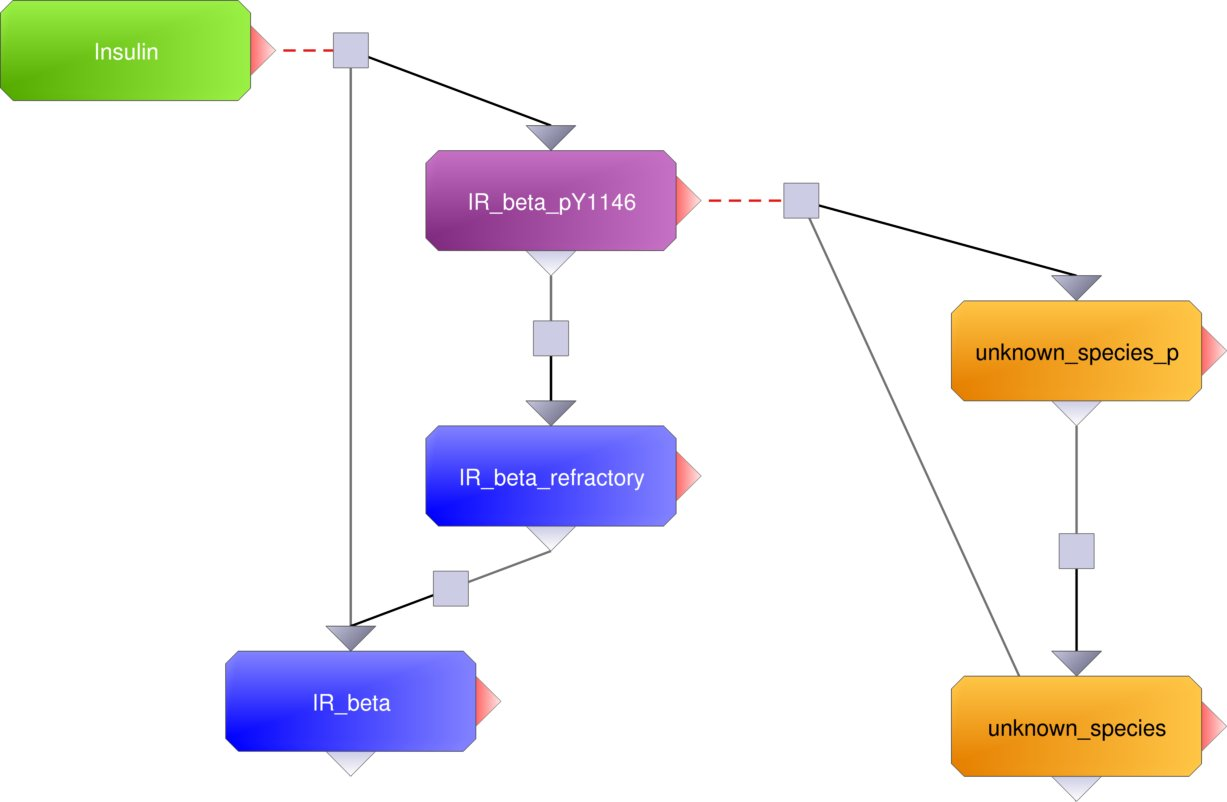
\includegraphics[scale=1.2]{insulin_receptor.jpg}
% 		\hfill
% 		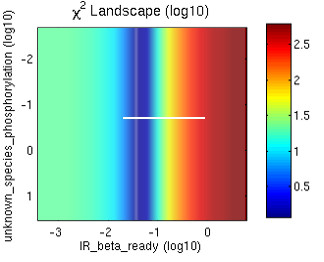
\includegraphics[scale=0.70]{structural_nonidentifiability_new.jpg}
% 		\textbf{B}
% 		\hfill
% 		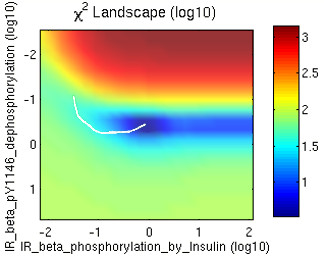
\includegraphics[scale=0.70]{practical_nonidentifiability_new.jpg}
% 		\textbf{C}
% 		\hfill
% 		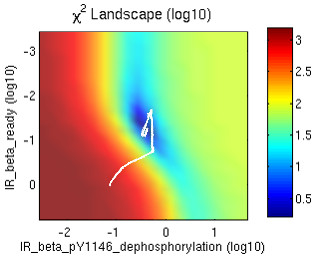
\includegraphics[scale=0.70]{identifiability_new.jpg}
% 		\textbf{D}
% 		\hfill
 		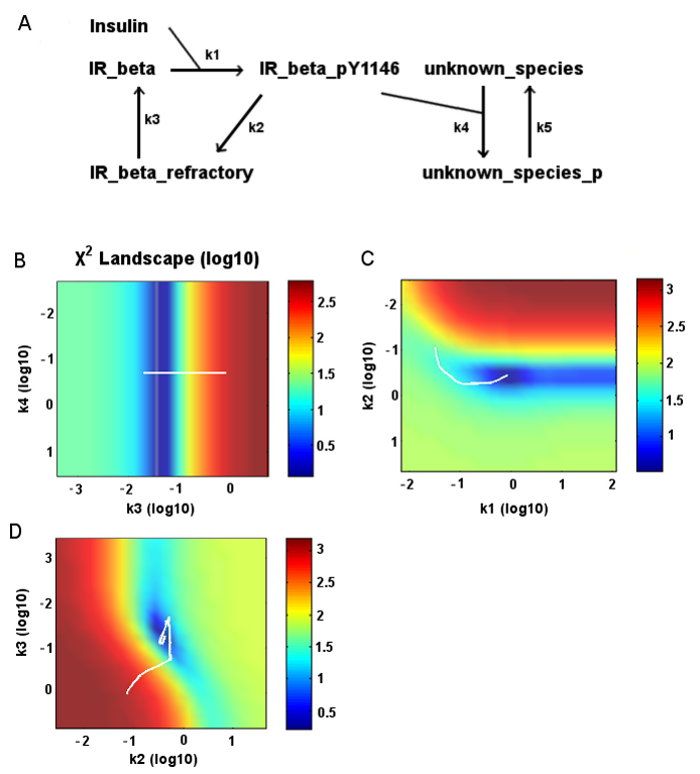
\includegraphics[width=350px]{ir_beta_model_identifiability.png}
		\caption[Graphical visualisation of parameter non-identifiability]{Graphical visualisation of parameter non-identifiability by $\log_{10}(\chi^2)$ landscape (darker colour correspond to parameter minimum). (A) Graphical mini-model of the insulin receptor with an additional unknown species. In this example, the only observable species is IR\_beta\_pY1146 which is phosphorylated by Insulin. IR\_beta\_pY1146 is responsible for the phosphorylation of unknown\_species, a species for which no information is available. (B) Structural non-identifiability for the parameter regulating the phosphorylation of unknown\_species. This parameter is clearly structurally non-identifiable as its dynamics are not mapped by any data. This parameter does not affect the search of solutions in the $\log_{10}(\chi^2)$ landscape. (C) Practical non-identifiability shown as an infinite upper bound confidence interval slightly above the parameter minimum (see blue $\chi^2$ region on the right). (D) Parameter identifiability. The 
parameter is clearly identifiable showing a well defined minimum and a confidence region. White line indicates the convergence path to a solution in the $\log_{10}(\chi^2)$ landscape.}
		\label{fig:landscape_identifiability}
	\end{center}
\end{figure}

\begin{figure}[tb]
	\begin{center}
		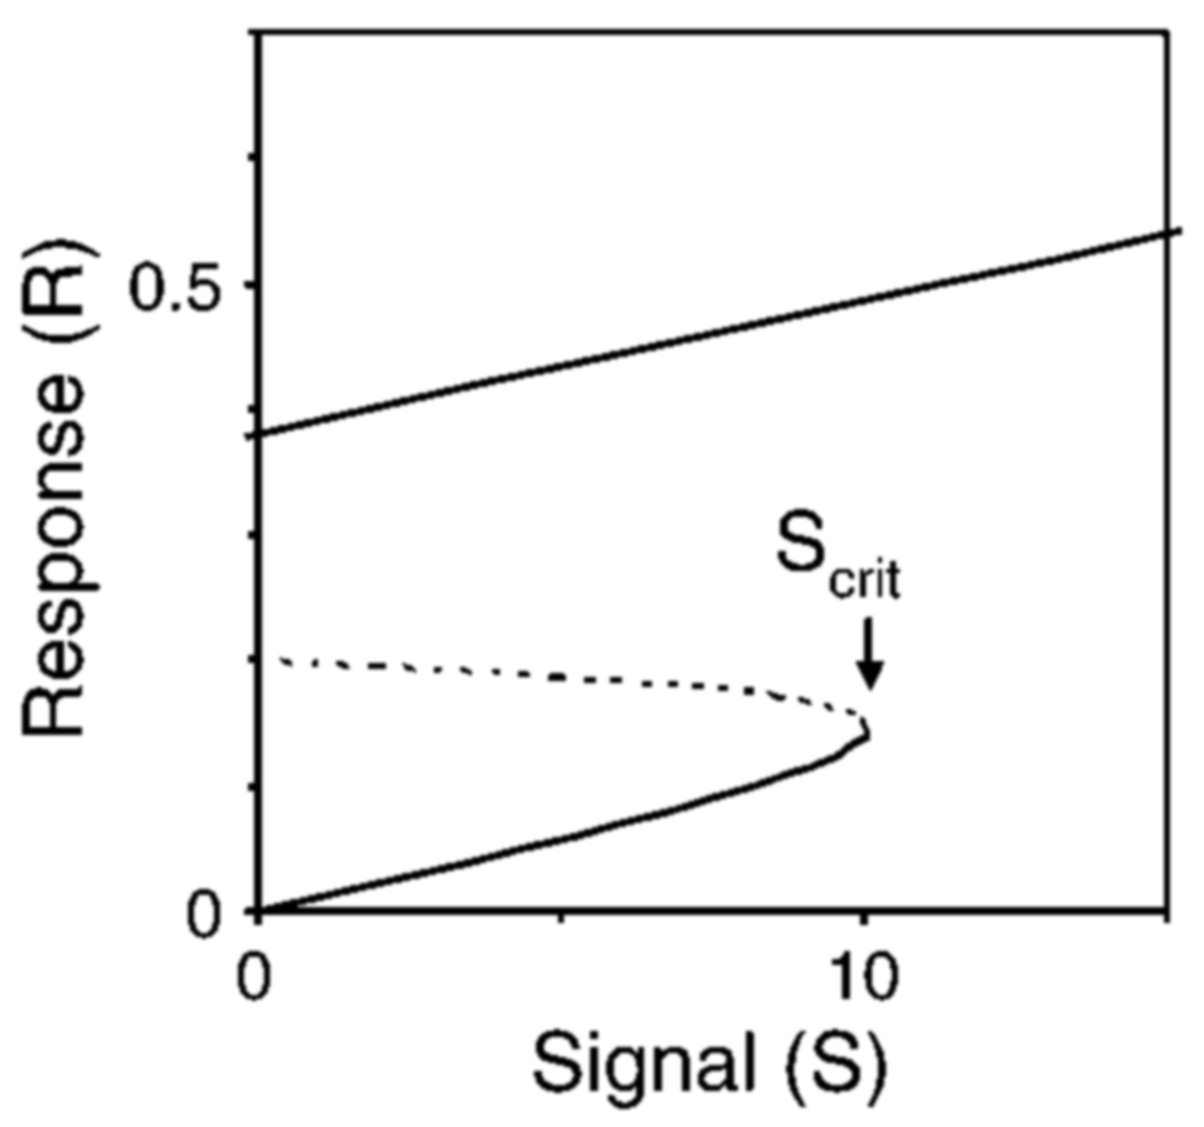
\includegraphics[scale=0.2]{tyson2003_fig1_adapted1.jpg}
		\textbf{A}
		\hfill
		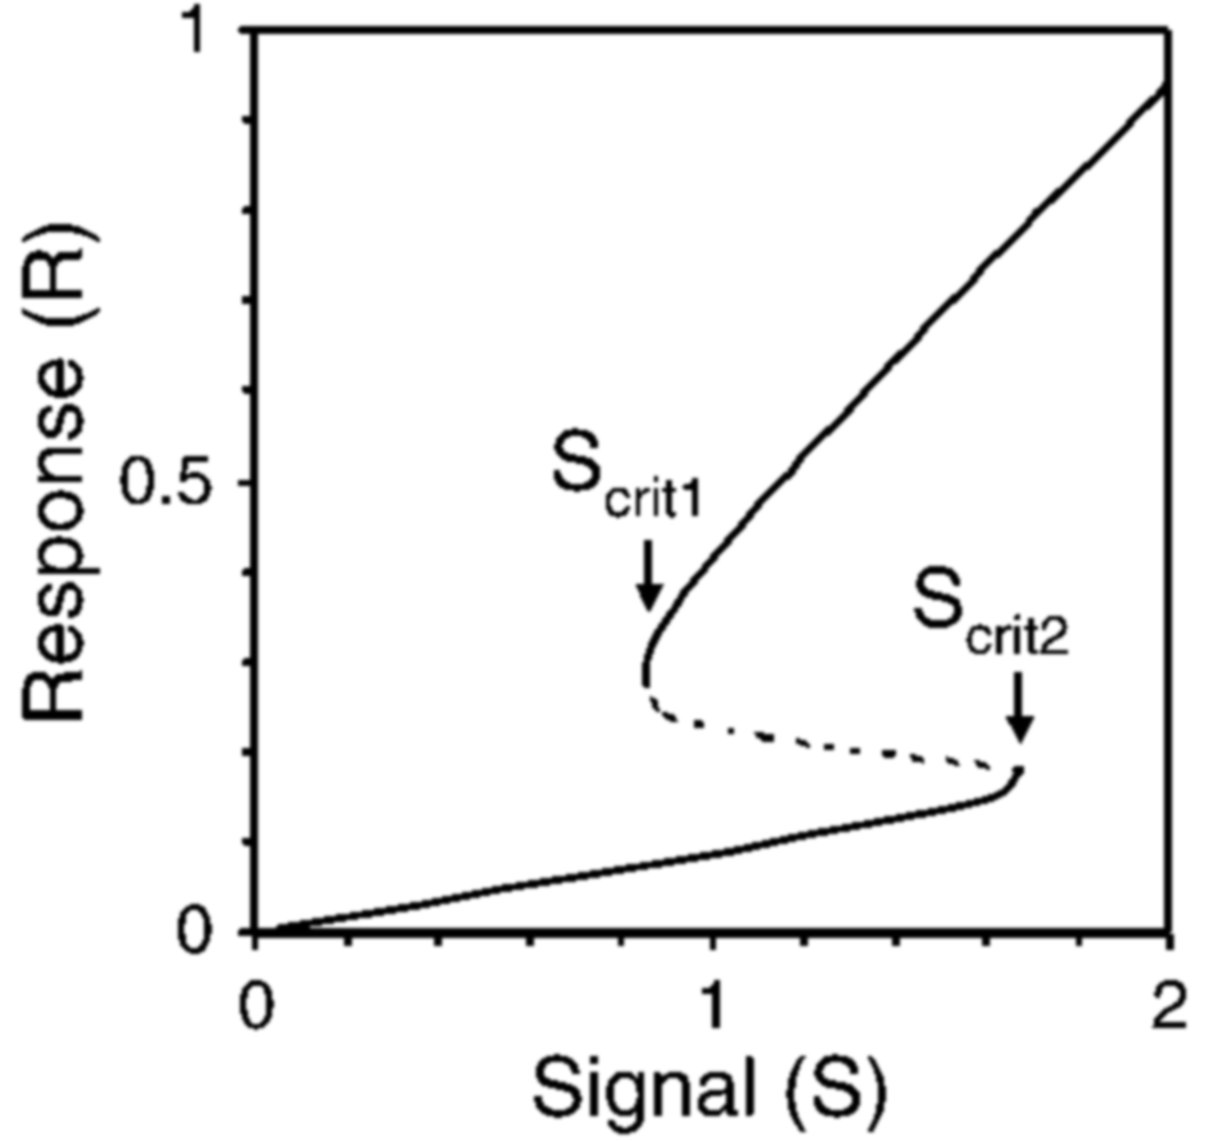
\includegraphics[scale=0.2]{tyson2003_fig1_adapted2.jpg}
		\textbf{B}
		\hfill
		\caption[Graphical examples of bifurcations.]{Graphical examples of bifurcations. (A) One-way switch bifurcation. At low levels of input stimulus, the system shows a bistable signalling response. After reaching a critical point, or bifurcation point, $S_{crit}$, the previous response dramatically changes into a monostable elevated response. This signalling response is characterised by two steady states (a low one and a high one) separated by an unstable state. However, the high steady state is the only one which persist above a certain threshold $S_{crit}$ of input stimulus, since the system is not able to restore its signalling response to the low steady-state. (B) Two-way toggle switch bifurcation. This type of bifurcation presents two bifurcation points, called $S_{crit1}$ and $S_{crit2}$, depending on both the strength and history of the input stimulus. This dependency of the response on the previous and current levels of the input stimulus represents the reason why these switches are also called \emph{
hysteresis}. In contrast to the previous case, this bifurcation permits to free the system from a constitutively activated response, since this one can be reduced by altering the signal strength. Adapted from \citep[Fig. 1]{Tyson2003}.}
		\label{fig:tyson2003_fig1_adapted}
	\end{center}
\end{figure}


\clearpage



%%% Local Variables: 
%%% mode: latex
%%% TeX-master: "../thesis"
%%% End: 
